\documentclass[]{scrartcl}
\title{Vorlesung Analysis II}
\usepackage{amsmath,amssymb,amsfonts}
\usepackage{stmaryrd}
\usepackage{mathtools}
\usepackage{latexsym}
\usepackage{graphicx}
\usepackage{tikz}
\usepackage{xcolor}
\usepackage{soul}
\usepackage{hyperref}
\usepackage{tipa}
\usepackage[dvipsnames]{xcolor}
\hypersetup{
	colorlinks=true,
	linkcolor=blue,
	filecolor=magenta,      
	urlcolor=cyan,
	pdftitle={Overleaf Example},
	pdfpagemode=FullScreen,
}
\newcommand{\redcircle}[1]{%
	\tikz[baseline=(char.base)]{
		\node[shape=circle, draw=red, text=red, thick, inner sep=1pt] (char) 
		{\textbf{#1}};
	}%
}
\setul{1pt}{3pt} % Linienhöhe und Abstand zum Text (optional anpassbar)

\setlength{\topmargin}{-.5in} \setlength{\textheight}{9.25in}
\setlength{\oddsidemargin}{0in} \setlength{\textwidth}{6.8in}
\setlength{\parindent}{0pt}

\begin{document}
	
	\textbf{\underline{Teil 2: topologische grundbegriffe in metrischen Räumen}}\\
	\\
	\textbf{\underline{an11: Topologische Grundbegriffe}}\\
	\\
	\textbf{\underline{\underline{Stichworte:} Umgebungsbasis, haisdorffsch, offen/abgeschlossen, Topologie}}\\
	\\
	\textbf{\underline{Literatur:}} \setulcolor{blue}\ul{[Forster], Kapitel 2}\\
	\\
	
	\textbf{11.1 \underline{Einleitung}}:\\
	Die bekannten Konzepte von "Kugel" und "Umgebung" können im metrischen Raum definiert und studiert werden. Die mehrdimensionale Analysis hat es oftmals erfordert, dass um ein Punkt $a\in D \subseteq\mathbb{R}^n$ immernoch eine Komplette Umgebung von a in D enthalten ist. Wir verallgemeinern dies für metrische Räume und kommen so zum Konzept offener und abgeschlossener Mengen, das zentral für die Topologie (als teilgebiet der Mathematik) ist.\\
	\\
	\textbf{11.2 \underline{Bezeichung}}: Sei $(R,\delta)$ metrischer Raum, sei $a\in R$, sei $\epsilon \textgreater0.$\\
	Dann heißt\setulcolor{yellow} \ul{$B_a^\epsilon$}:=$\{x\in R; \delta(x,a)\textless \epsilon\}$ eine \setulcolor{red}\ul{$\epsilon$-Umgebung} von a, ("Ball", "Kugel"...)\\
	und \setulcolor{yellow}\ul{$\tilde{\mathcal{U}_a}$}:=$\{U\subseteq R; U; U = B_a^\epsilon, \epsilon \textgreater 0 \text{geeignet}\}$\\
	heißt eine \setulcolor{red}\ul{Umgebungsbasis} von a.\\
	\underline{Bem.:}$ \tilde{\mathcal{U}}_a$ ist die Menge aller $ßepsilon$-Umgebungen von a, die in R enthalten sind.\\
	\\
	\textbf{11.3 \underline{Eigenschaften von $\epsilon$-Umgebungen}}:\\
	$(B0) \forall a \in R:$\setulcolor{green} \ul{$\tilde{\mathcal{U}_a}\neq\o$}, bzw. $\forall a \in R \exists B_a^\epsilon\in \tilde{\mathcal{U}_a}$,\\
	d-h- zu jedem Punkt $a\in R$ gibt es eine Umgebung von a in R.\\
	$(B1) \forall a \in R \forall B_a^\epsilon \in \tilde{\mathcal{U}_a}:$ \ul{$a \in B_a^\epsilon$}, d.h. jede Umgebung von a enthält a.\\
	$(B2) \forall a \in R \forall B_a^{\epsilon_1}, B_a^{\epsilon_2} \in \tilde{\mathcal{U}_a}:$ \ul{$B_a^{\epsilon_1}\cap B_a^{\epsilon_2}\in \tilde{\mathcal{U}_a}$}, und \ul{$B_a^{\epsilon_1}\cup B_a^{\epsilon_2}=B_a^{min(\epsilon_1,\epsilon_2)}$},\\
	d.h. der Durchschnitt zweier Umgebungen von a ist Umgebung von a.\\
	$(B3)\forall a,b \in R \forall $\ul{$B_a^\epsilon \ni b \exists V \in \tilde{\mathcal{U}_a}: V \subseteq B_a^\epsilon$},\\
	d.h. ist b in einer Umgebung U von a, so ex. eine Umgebung V von b mit V$\subseteq$U.\\
	\underline{Bew.:}
	\begin{figure}[h]
		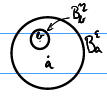
\includegraphics[width=2 cm,height=2cm]{bsp kap 11.3}
	\end{figure}\\
	\setulcolor{orange}\ul{$\eta:=\epsilon-\delta(a,b),$ sei $z\in B_a^\eta$}, d.h. $\delta(z,b)\textless \epsilon=\eta - \delta(a,b)\\ 
	\Rightarrow \delta(z,a)\leq \delta(z,b)+\delta(b,a)\textless \epsilon \Rightarrow z \in B_a^\epsilon\Rightarrow B_b^\eta \subseteq B_a^\epsilon$.\\
	\strut\hfill$\square$\\
	$(B4)\forall a,b \in R, a \neq b \exists U \in \tilde{\mathcal{U}_a}\exists V \in \tilde{\mathcal{U}_b}: $\setulcolor{green}\ul{U$\cap V =\o$},\\
	d.h. \ul{verschiedene Punkte} in T besitzen \ul{disjunkte Umgebungen}.\\
	Man nennt dies die \setulcolor{red}\ul{Trennungseigenschaft}, auch: R ist \ul{Hausdroff-Raum/hausdorffsch}\\
	$\rightarrow$"\ul{Hausdorffsches Trennungsaxiom"}/\ul{"T2-Trennungsaxiom"}\\
	\underline{Bew.:} 
	\begin{figure}[h]
		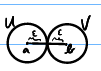
\includegraphics[width=2.5 cm,height=2cm]{bsp kap 11.3 2}
	\end{figure}\\
	Wähle $U=B_a^\epsilon, B_b^\epsilon mit$ \setulcolor{orange}\ul{$\epsilon=\frac{1}{2}\delta(a,b)$}.\\
	\strut\hfill$\square$\\
	\textbf{11.4} Fazit: \setulcolor{green} \ul{Metrische Räume sind hausdorffsch.}\\
	\\
	Eine leichte Verallgemeinerung ermöglicht es uns nun, von Umgebungen zu sprechen.\\
	\textbf{11.5 \underline{Def.:}} $U \subseteq R$ heißt \setulcolor{red} \ul{Umgebung von a}, falls $\exists B_a^\epsilon\subseteq U$.\\
	Setze \setulcolor{yellow} \ul{$U_a$:}= $\{U\subseteq R; B_a^\epsilon \subseteq U \text{ für geeignetes }\epsilon \textgreater 0\}$,\\
	die \setulcolor{red}\ul{Menge aller Umbegungen von a.}\\
	\underline{Bem.:}\setulcolor{blue}\ul{(B0)-(B4) in 11.3} gelten dann analog.\\
	\textbf{11.6 \underline{Def.:}}$U\subseteq R$ heißt \setulcolor{red}\ul{offen} (d.h. offenen Teilmenge), wenn $\forall_u \in U:U$ ist Umgebung von u.
	\textbf{11.7 \underline{Bsp.:}} \setulcolor{green} \ul{$B_a^\epsilon$ ist offen} wegen \setulcolor{blue} \ul{(B3)}.\\
	\\ 
	\textbf{11.8 \underline{Def.:}} Setze \setulcolor{yellow}\ul{$\mathcal{O}:$}= $\{U\leq R; U \text{offen}\}$, die \setulcolor{red}\ul{Mende aller offenen (Teil-)mengen von R.}\\
	\\
	\textbf{11.9 \underline{Bsp.:}} in $R=\mathbb{R}$ (als normierter VR bzgl. $|\cdot|$, dann also Raum bzgl. $\delta(x,y)=|x-y|$), sind offene Intervalle offene Mengen, aber auch beliebige Vereinigung offener Intervalle offen. Schnitte endlich vieler solcher offener Mengen sind wieder solche, nicht aber Schnitte unendlich vieler, denn z.B. ist \\
	$\bigcap_{\text{n}\in \mathbb{N}}]-\frac{-1}{n},\frac{1}{n}[=\{0\}$ keinbe offene Menge, obwohl alle IVe $]-\frac{-1}{n},\frac{1}{n}[$ offen sind.\\
	\\
	\textbf{11.10 \underline{Eigenschaften offener Mengen in R:}}\\
	$(\mathcal{O}_1) \o \in \mathcal{O}, $\setulcolor{green}\ul{$U_i\in \mathcal{O},i\in I \Rightarrow \bigcup_{i\in I} U_i \in \mathcal{O}$}, d.h. \o und die beliebige Vereinigung offener Mengen ist offen.\\
	\textopencorner Denn: $a\in \bigcup_{i\in I} U_i\Rightarrow ß\exists i\in I: a\in U\Rightarrow$ \setulcolor{orange}\ul{$B_a^{\epsilon_i}\subseteq U_i\subseteq\bigcup_{i\in I} U_i$.}\textcorner\\
	$(\mathcal{O}_2) R\in \mathcal{O},$ \setulcolor{green}\ul{$U_i \in \mathcal{O}, i\in \{1,...,n\}\Rightarrow\bigcup_{i\in I} U_i\in \mathcal{O}$}, d.h. der Schnitt endlich vieler offener Mengen ist offen.\\
	\textopencorner Denn: $\OE$ \setulcolor{orange}\ul{n=2(sonst VI)}. 
	\begin{figure}[h]
		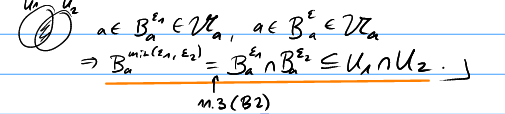
\includegraphics[width=8 cm,height=2.5cm]{bsp kap 11}
	\end{figure}\\
	\\
	\textbf{11.12 \underline{Bez.:}} Eine MEnge R mit einer Menge $\mathcal{O}$ von Teilmengen von R derart, dass die Eigenschaften $(O_1),(O_2)$ gelten, heißt \setulcolor{red}\ul{topologischer Raum.}\\
	In diesem Fall heißt$\mathcal{O}$ auch eine \ul{Topologie auf/von R}.\\
	Das Teilgebiet der Mathematik, in dem topologische Räume untersucht werden, nennt man \ul{Topologie}.\\
	\\
	\textbf{11.13 \underline{Beobachtung:}} Seien $||\cdot||^{(1)} \textbf{ und } ||\cdot||^{(2)}$ zwei Normen auf $\mathbb{R}^n$, nach \setulcolor{blue}\ul{10.10} sind diese äquivalent, d.h. $\exists\alpha,\beta\in \mathbb{R}:||\cdot||^{(1)} \leq \alpha||\cdot||^{2}\leq\beta||\cdot||^{1}.$\\
	Daraus folgt $\delta^{(1)} \leq \alpha\delta^{(2)}\leq \alpha\beta \delta^{(1)}$ für die zugehörige Metriken.\\
	Somit ist $(B_z^\epsilon)^{(1)} \supseteq \frac{1}{\alpha}(B_z^\epsilon)^{(2)}\supseteq \frac{1}{\alpha \beta}(B_z^\epsilon)^{(1)}$ für alle $z\in\mathbb{R}^n, \epsilon\textgreater0$,\\
	bzw.$(B_z^\epsilon)^{1}\subseteq\alpha(B_z^\epsilon)^{(2)}\subseteq\alpha\beta (B_z^\epsilon)^{(1)}$.\\
	Es ergibt sich,dass \setulcolor{green}\ul{$\mathcal{O}^{(1)}=\mathcal{O}^{(2)}$} ist, die von den beiden Normen induzierten Topologien sind also gleich! Zum Studium Topologischerr Fragen auf $\mathbb{R}^n$ fixiert man deswegen \underline{irgeneine} Norm $||\cdot||$
 	auf $\mathbb{R}^n$.\\
 	\\
 	Wir studieren im folgenden topologische Grundeigenschaften im metrischen Raum $(R,\delta)$\\
 	\textbf{11.14 \underline{Def.:}} Sei $M\subseteq R, a \in R$ geg.\\
 	Dann heißt a \setulcolor{red}\ul{Häufungspunkt von M} (kurz: \ul{HP von M})\\
 	$:\Leftrightarrow \forall U \in \mathcal{U}_a, (U\backslash\{a\})\cap M\neq \o.$ (Vgl. auch Def. in \setulcolor{blue}\ul{An 10.2}).\\
 	\\
 	\textbf{11.15 \underline{Bezeichnung:}}\setulcolor{yellow} \ul{$\dot{M}$}:= $\{a\in R; a \text{HP von M}\}$.\\
 	\\
 	\textbf{11.16 \underline{Def.:}} $M\subseteq R$ heißt \setulcolor{red}\ul{abgeschlossen} (Kurz:\ul{abg.}):$\Leftrightarrow$ \setulcolor{yellow}\ul{$\mathcal{C}M$}:= R$\backslash$M offen,\\
 	d.h. wenn $\mathcal{C}M$(das \setulcolor{red}\ul{Komplement von M}) in R eine offenen Teilmenge von R ist.\\
 	\\
 	\textbf{11.17 \underline{Bezeichnung:}} \setulcolor{yellow}\ul{$\mathcal{A}$}:= $\{M\subseteq R; \text{M Abgeschlossene Teilmenge von R}\}$\\
 	sei die Menge aller abg. Teilmengen von R.\\
 	\\
 	\textbf{11.18. Eigenschaften abgeschlossener Mengen:}\\
 	$(A_1) R\in\mathcal{A},$ \setulcolor{green}\ul{$A_i\in \mathcal{A}, i\in I \Rightarrow\bigcap_{i\in I}A_i \in \mathcal{A}$}, \textopencorner wegen($O_1$)\textcorner\\
 	d.h. R ist abg. und beliebige Durchschnitte abg. Mengen sind abg.\\
 	$(A_2)\o \in \mathcal{A},$ \ul{$A_i \in \mathcal{A},i\in\{1,...,n\}\Rightarrow \bigcup_{i=1}^{n}A_i \in \mathcal{A}$}, \textopencorner wegen($O_2$)\textcorner\\
 	d.h.\o ist abg. und endliche Vereinigungen abg. Mengen sind abg.\\
 	\\
 	\textbf{11.19 \underline{Bem.:}} \setulcolor{blue}\ul{($A_2$)} gilt nicht für unendlich viele $A_i$,\\
 	denn z.B. in $\mathbb{R}$ ist $\bigcup_{n\in \mathbb{N}}[\frac{1}{n},1]=]0,1]$ nicht abg., obwohl jedes Intervall $[\frac{1}{n}]$ abg. ist.\\
 	\textbf{11.20 \underline{Bem.:}} Es gibt Mengen, die (Gleichzeitig) offen \underline{und} abg. sind, z.B \o und R.\\
 	\\
 	\textbf{11.21 \underline{Bem.:}} Für $M\subseteq R$ gilt: \setulcolor{green} \ul{$M\in \mathcal{A} \Leftrightarrow \dot{M}\subseteq M$}.\\
 	\underline{Bew.:} 
 		\begin{align}
 			M\in \mathcal{A} &\Leftrightarrow \mathcal{C}M\in \mathcal{O} \Leftrightarrow \forall a \in \mathcal{C}M \exists U \in \mathcal{U}_a&&:U \subseteq \mathcal{C}M&\\
 			&\Leftrightarrow \forall a \in \mathcal{C}M \exists U \in \mathcal{U}_a &&: U \cap \mathcal{U}=\o\\
 			&\Leftrightarrow""&&:(U\backslash\{a\})\cap M =\o&\\
 			&\Leftrightarrow \mathcal{C}M\subseteq\mathcal{C}\dot{M}\Leftrightarrow\dot{M}\subseteq M&
 		\end{align}

	\hfill$\square$\\
	\textbf{11.22 \underline{Def.:}} Sei $M \subseteq R, a\in R.$\\
	Der Punkt a heißt \setulcolor{red}\ul{innerer Punkt von M} $\Leftrightarrow \exists U \in \mathcal{U}_a:U\subseteq M.$ (vgl. \setulcolor{blue} \ul{an 4.2})\\
	\\
	\textbf{11.23 \underline{Def.:}} Sei $M \subseteq R$, dann heißt \setulcolor{yellow} \ul{$\mathring{M}$ oder auch $M^o$}:=$\{a\in R,\text{a innerer Punkt von M}\}$ das \setulcolor{red}\ul{Innere von M}\\
	und $\overline{M}:=\{a\in R; \forall \epsilon \textgreater 0: B_a^\epsilon \cap M \neq\o\}$ die \setulcolor{red}\ul{Menge Der Berührungspunkte von M}.\\
	\\
	\textbf{11.24 \underline{Bem.:} $\mathring{M}$} ist die maximale offene Teilmenge von M,\\
	d.h. \setulcolor{green}\ul{$\mathring{M}$ offen} und (\ul{$\mathring{M}\subseteq \tilde{M}\subseteq M$ mit $\tilde{M}$ offen $\rightarrow\mathring{M}=\tilde{M}$}).\\
	Es folgt: \ul{M=$\mathring{M} \Leftrightarrow M$ offen}.\\
	\\
	\textbf{11.25 \underline{Bew.:}}$\cdot$ \setulcolor{orange}\ul{$\mathring{M}$} = 
	$\{a\in R ; \exists \epsilon_{a}\textgreater 0:B_a^{\epsilon_{a}}\subseteq M\}=$ \ul{$\bigcup_{a\in \mathring{M}}\underbrace{B_a^{\epsilon_{a}}}_{\text{offen}}$ ist offen.}\\
	$\cdot"M=\mathring{M}\Rightarrow M$ offen" ist klar, da $\mathring{M}$ offen.\\
	$\cdot$ Sei M offen, d.h. $\forall a \in M \exists \epsilon_{a}\textgreater 0: B_a^{\epsilon_{a}}\subseteq M \Rightarrow a \in M\mathring{M},$ also ist \ul{;$\subseteq$ $\mathring{M}$}.\\
	Da \ul{$\mathring{M}\subseteq$ M} klar ist, folgt M = $\mathring{M}$.\\
	\strut\hfill$\square$\\
	
	
	
	
		
	
\end{document} 
	